\documentclass[11pt]{article}

\usepackage{nmrdoc}
\usepackage{siunitx}
\usepackage{bm}
\usepackage{tikz}

\sisetup{per-mode=symbol}
\DeclareSIUnit{\angstrom}{\text{\AA}}
\DeclareSIUnit{\molar}{M}

\newcommand{\code}[1]{\texttt{#1}}
\setlength{\parindent}{0pt}
\setlength{\parskip}{0.42em}
\emergencystretch=2em

\begin{document}
\NmrTitle{Numerical Addendum: APBSField Calculator}

The APBS bridge performs the upstream solve: a linearized Poisson--Boltzmann
multigrid calculation on three equal grid dimensions read from
\code{apbs\_grid\_dim}, \(161^3\) in the default TOML. This addendum starts at
the boundary where that external solver returns a scalar potential grid
\(\phi\) in \(kT/e\). The calculator-owned numerics are the trilinear
interpolant over that grid, the nested central differences that form
\(\bm E=-\nabla\phi\) and \(\bm G=\partial\bm E/\partial\bm r\), the symmetric
traceless projection of \(\bm G\), and the shared \(T_2\) packing. The listings
below are distilled from the source: loops and bookkeeping are trimmed, but the
constants, guards, array shapes, and arithmetic are the implementation's.

\section{The cached potential grid}

\code{apbs\_solve} receives the atom count, coordinates, charges, PB radii, PB
parameters, grid-sizing arguments, and the three equal grid dimensions read
from \code{apbs\_grid\_dim}. It returns an \code{ApbsGridResult}; the C++ side keeps
only the origin \(\bm o\), the axis spacings
\(\bm h=(h_x,h_y,h_z)\), the integer dimensions \((n_x,n_y,n_z)\), and the flat
potential array. The flat index is \(x\)-fastest:
\[
  \code{idx}(x,y,z)=x+y\,n_x+z\,n_x n_y .
\]

\begin{codebox}
int grid_dim = static_cast<int>(CalculatorConfig::Get("apbs_grid_dim"));

ApbsGridResult apbs_grid;
int rc = apbs_solve(...,
                    grid_dim, grid_dim, grid_dim,
                    fine_dims[0], fine_dims[1], fine_dims[2],
                    coarse_dims[0], coarse_dims[1], coarse_dims[2],
                    &apbs_grid);
if (rc != APBS_BRIDGE_OK) {
    apbs_free_grid(&apbs_grid);
    return false;
}

grid.origin  = Vec3(apbs_grid.origin[0],
                    apbs_grid.origin[1],
                    apbs_grid.origin[2]);
grid.spacing = Vec3(apbs_grid.spacing[0],
                    apbs_grid.spacing[1],
                    apbs_grid.spacing[2]);
grid.dims[0] = apbs_grid.dims[0];
grid.dims[1] = apbs_grid.dims[1];
grid.dims[2] = apbs_grid.dims[2];
grid.data.assign(apbs_grid.data, apbs_grid.data + apbs_grid.n_points);
grid.valid = true;
\end{codebox}

The APBS grid is not asked for a field or a Hessian. Every derivative stored by
the calculator is recovered later from this scalar array.

\section{Trilinear interpolation}

For a requested point \(\bm p\), \code{GridCache::Interpolate} first converts
world coordinates to fractional grid coordinates,
\[
  u_d = \frac{p_d-o_d}{h_d},\qquad d\in\{x,y,z\}.
\]
The integer cell index is \(i_d=\lfloor u_d\rfloor\), and the in-cell fraction
is \(t_d=u_d-i_d\). The explicit \code{std::floor} matters: C++ integer
conversion truncates toward zero, so for \(u_x=-0.25\) it would choose cell
\(0\) and leave a negative blend weight, while \code{floor} chooses \(-1\) and
the out-of-grid guard rejects the point.

\begin{codebox}
for (int d = 0; d < 3; ++d)
    frac(d) = (point(d) - origin(d)) / spacing(d);

int ix = static_cast<int>(std::floor(frac(0)));
int iy = static_cast<int>(std::floor(frac(1)));
int iz = static_cast<int>(std::floor(frac(2)));

if (ix < 0 || ix >= dims[0]-1 ||
    iy < 0 || iy >= dims[1]-1 ||
    iz < 0 || iz >= dims[2]-1)
    return 0.0;

double fx = frac(0) - ix;
double fy = frac(1) - iy;
double fz = frac(2) - iz;
\end{codebox}

The blend is the tensor product of three one-dimensional linear blends. With
\(c_{\alpha\beta\gamma}=
\phi_{i_x+\alpha,i_y+\beta,i_z+\gamma}\) and
\(\alpha,\beta,\gamma\in\{0,1\}\), the interpolated value is
\[
  \Phi_h(\bm p)=
  \sum_{\alpha,\beta,\gamma}
  c_{\alpha\beta\gamma}\,
  w_x(\alpha)w_y(\beta)w_z(\gamma),
\]
where \(w_x(0)=1-t_x\), \(w_x(1)=t_x\), and likewise for \(y,z\). The source
writes the eight terms directly; the listing below only names the corner values
so the product structure is visible.

\begin{codebox}
auto idx = [&](int x, int y, int z) -> int {
    return x + y*dims[0] + z*dims[0]*dims[1];
};

double wx0 = 1.0 - fx, wx1 = fx;
double wy0 = 1.0 - fy, wy1 = fy;
double wz0 = 1.0 - fz, wz1 = fz;

double c000 = data[idx(ix,   iy,   iz  )];
double c100 = data[idx(ix+1, iy,   iz  )];
double c010 = data[idx(ix,   iy+1, iz  )];
double c110 = data[idx(ix+1, iy+1, iz  )];
double c001 = data[idx(ix,   iy,   iz+1)];
double c101 = data[idx(ix+1, iy,   iz+1)];
double c011 = data[idx(ix,   iy+1, iz+1)];
double c111 = data[idx(ix+1, iy+1, iz+1)];

return c000*wx0*wy0*wz0 + c100*wx1*wy0*wz0
     + c010*wx0*wy1*wz0 + c110*wx1*wy1*wz0
     + c001*wx0*wy0*wz1 + c101*wx1*wy0*wz1
     + c011*wx0*wy1*wz1 + c111*wx1*wy1*wz1;
\end{codebox}

If the grid is marked invalid, or if any of the eight required corners would
lie outside the stored array, the helper returns \(0.0\). The configured grid
padding is intended to keep atom-centered derivative stencils inside the grid;
this zero return is the fallback guard.

\section{Nested central differences}

The electric field is a centered difference of the interpolant
\(\Phi_h\), not a derivative returned by APBS. For component \(a\), the code
moves one grid spacing forward and backward along the same axis, interpolates
the potential at both displaced points, subtracts, divides by \(2h_a\), and
applies the electrostatic minus sign:
\[
  E_a(\bm r)=
  -\frac{\Phi_h(\bm r+h_a\hat{\bm e}_a)
          -\Phi_h(\bm r-h_a\hat{\bm e}_a)}
         {2h_a}.
\]

\begin{codebox}
static Vec3 ElectricFieldFromGrid(const GridCache& grid,
                                  const Vec3& point) {
    Vec3 E;
    for (int d = 0; d < 3; ++d) {
        Vec3 plus = point, minus = point;
        plus(d)  += grid.spacing(d);
        minus(d) -= grid.spacing(d);

        E(d) = -(grid.Interpolate(plus) - grid.Interpolate(minus))
               / (2.0 * grid.spacing(d));
    }
    return E;
}
\end{codebox}

The field-gradient matrix is then a centered difference of that computed field.
The column index \(j\) is the direction in which the field is perturbed; the row
index \(i\) is the component of \(\bm E\) being read:
\[
  G_{ij}(\bm r)=
  \frac{E_i(\bm r+h_j\hat{\bm e}_j)
        -E_i(\bm r-h_j\hat{\bm e}_j)}
       {2h_j}.
\]

\begin{codebox}
static Mat3 FieldGradientFromGrid(const GridCache& grid,
                                  const Vec3& point) {
    Mat3 EFG;
    for (int j = 0; j < 3; ++j) {
        Vec3 plus = point, minus = point;
        plus(j)  += grid.spacing(j);
        minus(j) -= grid.spacing(j);

        Vec3 Eplus  = ElectricFieldFromGrid(grid, plus);
        Vec3 Eminus = ElectricFieldFromGrid(grid, minus);

        for (int i = 0; i < 3; ++i)
            EFG(i, j) = (Eplus(i) - Eminus(i))
                        / (2.0 * grid.spacing(j));
    }
    ...
}
\end{codebox}

Expanding the nested calls shows how the potential values move. For \(i\ne j\),
one entry uses four interpolated potentials at the corners of a rectangle
around the atom:
\[
\begin{aligned}
  G_{ij}(\bm r) =
  \frac{
     -\Phi_h(\bm r+h_j\hat{\bm e}_j+h_i\hat{\bm e}_i)
     +\Phi_h(\bm r+h_j\hat{\bm e}_j-h_i\hat{\bm e}_i)}
       {4h_i h_j} \\[0.2em]
  +\frac{
      \Phi_h(\bm r-h_j\hat{\bm e}_j+h_i\hat{\bm e}_i)
     -\Phi_h(\bm r-h_j\hat{\bm e}_j-h_i\hat{\bm e}_i)}
       {4h_i h_j}.
\end{aligned}
\]
This is the mixed second difference of \(\Phi_h\), with the minus sign inherited
from \(\bm E=-\nabla\phi\). For \(i=j\), the code becomes
\[
  G_{ii}(\bm r)=
  -\frac{\Phi_h(\bm r+2h_i\hat{\bm e}_i)
          -2\Phi_h(\bm r)
          +\Phi_h(\bm r-2h_i\hat{\bm e}_i)}
         {4h_i^2}.
\]
Thus the diagonal second derivative is not the direct adjacent-point Hessian
stencil \((\Phi_{+h}-2\Phi_0+\Phi_{-h})/h^2\). It is the consequence of
differencing the field that was itself differenced from the potential.

\begin{figure}[ht]
\centering
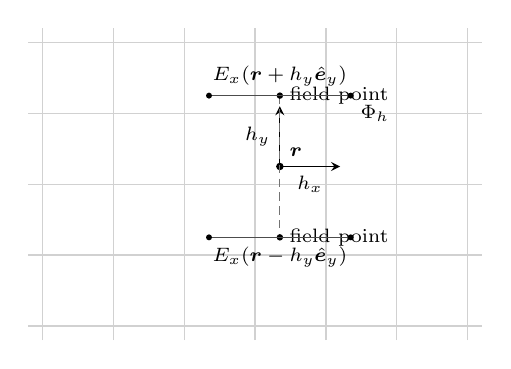
\begin{tikzpicture}[scale=0.9,line width=0.45pt,>=stealth]
  \foreach \x in {-3,-2,-1,0,1,2,3}
    \draw[black!18] (\x,-2.2) -- (\x,2.2);
  \foreach \y in {-2,-1,0,1,2}
    \draw[black!18] (-3.2,\y) -- (3.2,\y);

  \coordinate (R) at (0.35,0.25);
  \coordinate (Yp) at (0.35,1.25);
  \coordinate (Ym) at (0.35,-0.75);
  \coordinate (Ppp) at (1.35,1.25);
  \coordinate (Ppm) at (-0.65,1.25);
  \coordinate (Pmp) at (1.35,-0.75);
  \coordinate (Pmm) at (-0.65,-0.75);

  \fill (R) circle (1.5pt) node[above right] {\scriptsize \(\bm r\)};
  \draw[->] (R) -- +(0.85,0) node[midway,below] {\scriptsize \(h_x\)};
  \draw[->] (R) -- +(0,0.85) node[midway,left] {\scriptsize \(h_y\)};

  \draw[black!55,densely dashed] (Yp) -- (Ym);
  \fill (Yp) circle (1.3pt) node[right] {\scriptsize field point};
  \fill (Ym) circle (1.3pt) node[right] {\scriptsize field point};

  \draw[black!70] (Ppm) -- (Ppp);
  \draw[black!70] (Pmm) -- (Pmp);
  \fill (Ppp) circle (1.2pt);
  \fill (Ppm) circle (1.2pt);
  \fill (Pmp) circle (1.2pt);
  \fill (Pmm) circle (1.2pt);
  \node[above] at (0.35,1.25) {\scriptsize \(E_x(\bm r+h_y\hat{\bm e}_y)\)};
  \node[below] at (0.35,-0.75) {\scriptsize \(E_x(\bm r-h_y\hat{\bm e}_y)\)};
  \node[below right] at (1.35,1.25) {\scriptsize \(\Phi_h\)};
\end{tikzpicture}
\caption{A two-dimensional slice of the nested stencil for \(G_{xy}\). The
outer \(y\)-difference compares two field points; each field point is an
\(x\)-difference of two interpolated potentials. Each of the four potential
samples is itself an eight-corner trilinear blend in the full three-dimensional
grid.}
\end{figure}

The nesting also shows how interpolation error is differentiated. A field
component subtracts two interpolated values and divides by grid spacing; a
field-gradient entry subtracts two such field components and divides again. The
EFG therefore contains two finite-difference passes over the piecewise-trilinear
interpolant. Across cell faces the interpolant is continuous, but its derivative
is cell-dependent and can jump; the two mixed entries \(G_{ij}\) and \(G_{ji}\)
therefore need not agree to machine precision.

\section{Symmetric traceless projection}

The raw \(\bm G\) from the previous section is projected before storage. First,
the code replaces it by \(\tfrac12(\bm G+\bm G^{\mathsf T})\). That operation
sets the antisymmetric subspace to zero, so the shared decomposition has no
field-gradient \(T_1\) channel to report. Second, the code subtracts one third
of the computed trace from each diagonal entry:
\[
  \widetilde{\bm G}
  =
  \frac{\bm G+\bm G^{\mathsf T}}{2}
  -\frac{\operatorname{tr}\left[
        (\bm G+\bm G^{\mathsf T})/2\right]}{3}\bm I .
\]

\begin{codebox}
EFG = 0.5 * (EFG + EFG.transpose());

double trace = EFG.trace();
EFG -= (trace / 3.0) * Mat3::Identity();

return EFG;
\end{codebox}

Symmetrization removes the antisymmetric residue from finite differencing the
piecewise trilinear interpolant rather than differentiating a differentiable
potential. The trace is \(\nabla\cdot\bm E=-\Delta\phi\). Away from charge
density, the field-gradient matrix of external sources is traceless; at the
target atom, the APBS potential includes that atom's own Coulomb term, whose
Laplacian is a delta function. The grid represents that delta as a finite
diagonal average near the atom. Subtracting trace/3 from the diagonal removes
that average without changing the symmetric traceless part left for \(T_2\).

\section{Storage guards and units}

The projection above runs in APBS-native units. Afterward the per-atom path applies
finite-value guards, a field-only magnitude cap, and the thermal-voltage
conversion. If any component of \(\bm E\) is NaN or infinite, both \(\bm E\)
and \(\widetilde{\bm G}\) are set to zero. If \(\bm E\) is finite but its
native magnitude is greater than \code{APBS\_SANITY\_LIMIT}, \(100.0\) in
\(kT/(e\,\si{\angstrom})\), the vector is rescaled to that magnitude. The cap
does not rescale the EFG. Non-finite EFG entries that remain are zeroed one at
a time.

\begin{codebox}
Vec3 E = ElectricFieldFromGrid(grid, pos);
Mat3 EFG = FieldGradientFromGrid(grid, pos);

if (E_has_nan_or_inf) {
    E = Vec3::Zero();
    EFG = Mat3::Zero();
} else {
    double E_mag = E.norm();
    if (E_mag > APBS_SANITY_LIMIT)
        E *= APBS_SANITY_LIMIT / E_mag;
}

for (int a = 0; a < 3; ++a)
    for (int b = 0; b < 3; ++b)
        if (std::isnan(EFG(a,b)) || std::isinf(EFG(a,b)))
            EFG(a,b) = 0.0;

E   *= KT_OVER_E_298K;
EFG *= KT_OVER_E_298K;
\end{codebox}

\code{KT\_OVER\_E\_298K} is \(0.025693\) volts in
\code{src/PhysicalConstants.h}. The conversion uses this fixed 298.15 K
constant, not a value recomputed from the runtime APBS temperature; the default
TOML temperature is also 298.15 K. Multiplication by it turns
\(kT/(e\,\si{\angstrom})\) into \(\si{\volt\per\angstrom}\), and
\(kT/(e\,\si{\angstrom\squared})\) into
\(\si{\volt\per\angstrom\squared}\). The stored atom fields are the converted
\(\bm E\) and \(\widetilde{\bm G}\).

\section{The shared tensor projection}

The field-gradient matrix then passes through
\code{SphericalTensor::Decompose}. The routine is closed-form arithmetic:
trace to \(T_0\), antisymmetric differences to \(T_1\), and the symmetric
traceless part to the five \(T_2\) components.

\begin{codebox}
st.T0 = sigma.trace() / 3.0;

st.T1[0] = 0.5*(sigma(1,2) - sigma(2,1));
st.T1[1] = 0.5*(sigma(2,0) - sigma(0,2));
st.T1[2] = 0.5*(sigma(0,1) - sigma(1,0));

double Sxx = sigma(0,0) - st.T0;
double Syy = sigma(1,1) - st.T0;
double Szz = sigma(2,2) - st.T0;
double Sxy = 0.5*(sigma(0,1) + sigma(1,0));
double Sxz = 0.5*(sigma(0,2) + sigma(2,0));
double Syz = 0.5*(sigma(1,2) + sigma(2,1));

st.T2[0] = std::sqrt(2.0)     * Sxy;
st.T2[1] = std::sqrt(2.0)     * Syz;
st.T2[2] = std::sqrt(3.0/2.0) * Szz;
st.T2[3] = std::sqrt(2.0)     * Sxz;
st.T2[4] = (Sxx - Syy) / std::sqrt(2.0);
\end{codebox}

The \(\sqrt2\) factors on off-diagonals make the five-vector length equal the
Frobenius length of the symmetric traceless matrix: an off-diagonal entry
\(S_{xy}\) appears twice in a symmetric \(3\times3\) matrix, and
\((\sqrt2 S_{xy})^2\) accounts for both entries. The two diagonal coordinates
\(\sqrt{3/2}S_{zz}\) and \((S_{xx}-S_{yy})/\sqrt2\) account for the three
diagonal entries under the constraint \(S_{xx}+S_{yy}+S_{zz}=0\).

For APBSField, the input to this routine has already been symmetrized and
de-traced. Thus \(T_1\) is zero by construction, and \(T_0\) is zero up to the
roundoff in the trace subtraction. \code{apbs\_E.npy} stores the Cartesian
field as \((N,3)\); \code{apbs\_efg.npy} stores only the five \(T_2\) entries as
\((N,5)\).

\section{Glossary}

\textbf{Trilinear interpolation.} A point inside a grid cell borrows from the
eight surrounding corners, the nearer corners carrying more of the value (the
weights set by the fractional distances to each corner). At the centre of a cell
all eight weights are \(1/8\); at a cell
corner one weight is \(1\) and the other seven are \(0\). Formally, it is the
tensor product of three linear interpolants over the unit cube, producing a
continuous piecewise-polynomial \(\Phi_h(\bm p)\).

\textbf{Central finite difference.} A slope read by stepping the same distance
to either side of a point and dividing the rise by the run (the function
evaluated symmetrically across the point, the signed change divided by the full
separation). The APBS field component \(E_x\) uses
\(\Phi_h(\bm r+h_x\hat{\bm e}_x)\) and
\(\Phi_h(\bm r-h_x\hat{\bm e}_x)\), with the electrostatic minus sign.
Formally, the first derivative approximation is
\([f(x+h)-f(x-h)]/(2h)\), with the APBS EFG applying the same operation once
again to the computed field.

\textbf{Traceless (deviatoric) projection.} Drop a matrix's uniform swell and
keep the part that stretches some directions while compressing others (its
zero-trace part, recovered by subtracting the spherical average from the
diagonal). For
\(\operatorname{diag}(2,-1,-1)\) the trace is already zero, while
\(\operatorname{diag}(3,3,3)\) projects to zero. Formally, the projection maps
\(\bm A\) to \(\bm A-\operatorname{tr}(\bm A)\bm I/3\).

\textbf{Spherical tensor \(T_2\).} The pure stretch-and-squeeze of a
\(3\times3\) tensor --- pulled out along some directions, pushed in along others,
averaging to nothing (its traceless symmetric part, packed into five
isometrically normalized components). In
APBSField it is the exported field-gradient feature, so the stored numbers
describe the rank-2 part of the local electric-field gradient, not a chemical
shift. Formally, \(T_2\) is the five-number traceless symmetric block of the
tensor's nine components, with the basis isometrically normalized to preserve
the Frobenius norm.

\end{document}
